% Created 2023-12-14 Thu 13:22
% Intended LaTeX compiler: pdflatex
\documentclass[a4paper,11pt]{article}
\usepackage[utf8]{inputenc}
\usepackage[T1]{fontenc}
\usepackage{graphicx}
\usepackage{longtable}
\usepackage{wrapfig}
\usepackage{rotating}
\usepackage[normalem]{ulem}
\usepackage{amsmath}
\usepackage{amssymb}
\usepackage{capt-of}
\usepackage{hyperref}
\usepackage{listings}
\usepackage{lipsum}
\usepackage{subcaption}
\usepackage{caption}
\usepackage{float}
\hypersetup{hidelinks}
\usepackage[section]{placeins}
\usepackage[format=hang, width=.85\textwidth]{caption}
\usepackage[margin=1.3in]{geometry}
\author{Oskar Haukebøe}
\date{\today}
\title{Detection of shared network bottleneck using passive WiFi traffic analysis\\\medskip
\large IN3260}
\hypersetup{
 pdfauthor={Oskar Haukebøe},
 pdftitle={Detection of shared network bottleneck using passive WiFi traffic analysis},
 pdfkeywords={},
 pdfsubject={},
 pdfcreator={Emacs 29.0.91 (Org mode 9.7-pre)}, 
 pdflang={English}}
\usepackage{calc}
\newlength{\cslhangindent}
\setlength{\cslhangindent}{1.5em}
\newlength{\csllabelsep}
\setlength{\csllabelsep}{0.6em}
\newlength{\csllabelwidth}
\setlength{\csllabelwidth}{0.45em * 3}
\newenvironment{cslbibliography}[2] % 1st arg. is hanging-indent, 2nd entry spacing.
 {% By default, paragraphs are not indented.
  \setlength{\parindent}{0pt}
  % Hanging indent is turned on when first argument is 1.
  \ifodd #1
  \let\oldpar\par
  \def\par{\hangindent=\cslhangindent\oldpar}
  \fi
  % Set entry spacing based on the second argument.
  \setlength{\parskip}{\parskip +  #2\baselineskip}
 }%
 {}
\newcommand{\cslblock}[1]{#1\hfill\break}
\newcommand{\cslleftmargin}[1]{\parbox[t]{\csllabelsep + \csllabelwidth}{#1}}
\newcommand{\cslrightinline}[1]
  {\parbox[t]{\linewidth - \csllabelsep - \csllabelwidth}{#1}\break}
\newcommand{\cslindent}[1]{\hspace{\cslhangindent}#1}
\newcommand{\cslbibitem}[2]
  {\leavevmode\vadjust pre{\hypertarget{citeproc_bib_item_#1}{}}#2}
\makeatletter
\newcommand{\cslcitation}[2]
 {\protect\hyper@linkstart{cite}{citeproc_bib_item_#1}#2\hyper@linkend}
\makeatother\begin{document}

\maketitle

\section{Introduction}
\label{sec:org62263d0}
Network performance issues are a widespread nuisance that can often leave users perplexed about their origin—be it within their local WiFi or due to external factors such as distant servers. Identifying these bottlenecks is critical in maintaining a proficient network experience.

One project that attempts to solve this challenge is NETHINT \cslcitation{1}{[1]}, which leverages passive WiFi traffic analysis to evaluate latency and packet loss, providing insights into whether the congestion lies in the local network or not.

This assignment builds upon the work of NETHINT by empirically testing its capability to discern the location of bottlenecks within a controlled environment. Utilization of a TEACUP \cslcitation{2}{[2]} testbed facilitates a systematic approach to simulating various network scenarios with different points of congestion. Through automated experiments on real machines, this assignment aims to critically evaluate NETHINT's proficiency in accurately identifying whether local WiFi is the limiting factor. The TEACUP configuration used is available at \cslcitation{3}{[3]}.
\section{Testbed configuration}
\label{sec:org3f8c0f3}
The primary distinctive feature of NETHINT is its utilization of passive network measurements, ensuring no interference with the network \cslcitation{4}{[4]}. It achieves this by monitoring WiFi traffic and analyzing packet timings for each device on the network. This allows for a comparative assessment of the packet delay across different devices, which then can be used to determine whether the devices on the network have a common bottleneck or not. Should a common bottleneck be identified, it likely indicates that congestion exists within the local area network (LAN).

To assess NETHINT's ability to recognize local WiFi bottlenecks, we configure a network topology as shown in Figure \ref{fig:orga947e73}. All nodes in this topology are physical computers running Debian Linux, aside from the switch. They are managed by another computer not depicted in the figure, using TEACUP. This setup enables automated generation of network traffic, as well as throughput and delay limitations at the routers. Additionally, it enables automatic logging of network traffic.

\begin{figure}[t]
\centering
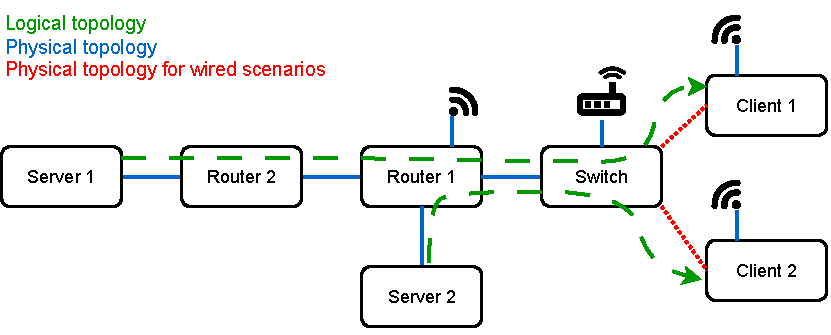
\includegraphics[width=.9\linewidth]{figures/topology-wireless.drawio-1.pdf}
\caption{\label{fig:orga947e73}Topology of the testbed}
\end{figure}
\subsection{Network Devices and Configuration}
\label{sec:org841c63f}
Figure \ref{fig:orga947e73} shows how all the devices are connected, and how the traffic flows between them. The logical topology shows how the traffic between Server~1 and Client~1 passes both routers, while the traffic between Server~2 and Client~2 only passes one router. This allows us to position the bottleneck at either Router 1 or Router 2, which gives either a shared bottleneck or no shared bottleneck between the two logical topologies. The roles of the individual nodes are the following:

\begin{itemize}
\item \emph{Servers:} Two servers (Server~1 and Server~2) for generating traffic.
\item \emph{Clients:} Two clients (Client~1 and Client~2) to act as traffic endpoints.
\item \emph{Routers:} Two routers with Router 1 being the entry point for both clients. Network congestion is generated at the routers.
\item \emph{Switch:} A switch to connect the clients with Router 1, enabling bandwidth limitation at the router level.
\item \emph{WiFi AP:} An access point for the wireless segment of the network, set to channel 3 without encryption to accommodate NETHINT's capabilities.
\item \emph{WiFi interface at Router 1:} Router 1's WiFi card, set to monitor mode for traffic sniffing, also configured to channel 3 to monitor the WiFi AP.
\end{itemize}

This setup models a scenario where Client~2 consumes VoIP traffic from Server~2, while Client~1 consumes bandwidth for different activities from Server~1. The objective is to determine whether NETHINT is able to discern whether  traffic between Server~1 and Client~1 interferes with the traffic between Server~2 and Client~2.
\subsubsection{Address configuration}
\label{sec:org5f037ec}
We use a switch to connect the two clients to the first router, allowing both clients to access Router 1 through the same network interface for wired connections. This setup facilitates bandwidth limitation at the router, enabling both clients to share the available bandwidth.

The WiFi AP is also connected to the switch and provides an unencrypted WiFi network. The lack of encryption is due to NETHINT's inability to decrypt WiFi traffic. Both clients connect to this network, thus gaining access to the two servers over WiFi. Router 1's WiFi card, configured in monitor mode, is used by NETHINT to capture all the WiFi traffic between the clients and the WiFi AP. To enable traffic monitoring, the WiFi interface on Router 1 and the WiFi AP are both set to channel 3.

For the machines to recognize how to reach each other, they had to be configured to know where the packets should be sent. Client~2, for example, was configured in the file \texttt{/etc/network/interfaces.d/vlan11-iface} as follows:
\begin{lstlisting}[basicstyle=\ttfamily\footnotesize,breaklines=true,showstringspaces=false,postbreak=\mbox{$\hookrightarrow$\space},tabsize=2,language=sh,numbers=none]
auto enp36s0
iface enp36s0 inet static
      address 172.16.12.5/24
      up route add -net 172.16.10.0 netmask 255.255.255.0 gw 172.16.12.254 || true
      up route add -net 172.16.11.0 netmask 255.255.255.0 gw 172.16.12.254 metric 10 || true
      up route add -net 10.10.12.0 netmask 255.255.255.0 gw 172.16.12.254 metric 10 || true
\end{lstlisting}

The IP address \texttt{172.16.12.254} corresponds to the network interface of Router 1 that faces the switch. The address \texttt{172.16.11.0} is linked with Server~2, and \texttt{10.10.12.0} with Server~1. This configuration indicates to Client~2 that it can reach the servers via Router 1. The address \texttt{172.16.10.0} represents the interface on Router 1 facing Router 2 and was necessary for TEACUP operations, as it requires initial ping tests between certain nodes.

While the above outlines wired connectivity, the main tests needed to run wirelessly, hence the specification of \texttt{metric 10} in the routing commands. Given that clients can reach servers both via the WiFi AP and via the wired connections, it is crucial to ensure they utilize the correct network path. The following commands configure client preferences for network interfaces:
\begin{lstlisting}[basicstyle=\ttfamily\footnotesize,breaklines=true,showstringspaces=false,postbreak=\mbox{$\hookrightarrow$\space},tabsize=2,language=sh,numbers=none]
sudo ip route add 172.16.11.0/24 via 172.16.13.1 metric 2
sudo ip route del 172.16.11.0/24 via 172.16.13.1 meric 2
\end{lstlisting}

Here, \texttt{172.16.13.1} is the IP of the WiFi AP. These commands alternate the traffic route between the wired and wireless interfaces on the clients, allowing us to easily switch between running the tests over WiFi or over Ethernet.
\subsection{Bottleneck configuration}
\label{sec:org2899799}
The bottlenecks are placed at either Router 1, Router 2, or at the WiFi AP. This corresponds to the two users at Client~1 and Client~2 either having a common bottleneck or not. When the bottleneck occurs at Router 2, the user at Client~2 is not expected be significantly affected, as Router 1 should still have a surplus of bandwidth.
\subsubsection{Configuration of throughput limitations}
\label{sec:orgdf2a4b4}
In order to configure the bottlenecks, we change the capacity at Router 1 and Router 2. The throughput at the WiFi AP is set to the lowest value it supports, which is 54 Mbps. Depending on the desired bottleneck location, the capacity at Router 1 and Router 2 was adjusted either above or below this threshold. Table \ref{tab:org6a6e085} lists capacity values used in each bottleneck scenario.

\begin{table}[htbp]
\caption{\label{tab:org6a6e085}Configured capacity at the two routers in the different bottleneck configurations}
\centering
\begin{tabular}{lrr}
Bottleneck at: & Router 1 (Mbps) & Router 2 (Mbps)\\[0pt]
\hline
Router 1 & 15 & 70\\[0pt]
Router 2 & 70 & 15\\[0pt]
WiFi AP & 70 & 70\\[0pt]
\end{tabular}
\end{table}
\subsubsection{Additional variable adjustments}
\label{sec:org8f1668c}
In addition to throughput, both queue length and delay were varied on Router 1. The queue lengths were:
\begin{itemize}
\item 0.5 BDP
\item 1 BDP
\item 1.5 BDP
\item 2 BDP
\end{itemize}

Delays of 50ms and 10ms were tested at Router 1, with Router 2 consistently set at a 10ms delay. The actual buffer sizes used for the tests are listed in Table \ref{tab:orge6eaa93}. These values were calculated using 15Mbps as the lowest capacity. However, an oversight led us to not update these values for when the WiFi AP was the bottleneck where the lowest throughput was 45Mbps. This caused the BDP values used for this traffic to be around \(\frac{1}{3}\) of what it was supposed to be.

\begin{table}[htbp]
\caption{\label{tab:orge6eaa93}Buffer sizes used on Router 1 (in number of packets) for the different delay and bdp configurations}
\centering
\begin{tabular}{lrr}
 & 10ms delay & 50ms delay\\[0pt]
\hline
0.5 BDP & 6 & 31\\[0pt]
1 BDP & 12 & 62\\[0pt]
1.5 BDP & 18 & 93\\[0pt]
2 BDP & 24 & 124\\[0pt]
\end{tabular}
\end{table}
\subsubsection{TEACUP configuration}
\label{sec:orge37d1a0}
In order to set these limitations, we used the built-in functions of TEACUP which allows us to set these limitations for one of the routers, and then it runs the tests for each of the values specified. This is done by setting the following variables in the TEACUP configuration:

\begin{lstlisting}[basicstyle=\ttfamily\footnotesize,breaklines=true,showstringspaces=false,postbreak=\mbox{$\hookrightarrow$\space},tabsize=2,language=Python,numbers=none]
# Emulated delays in ms
TPCONF_delays = [25,]

# Emulated bandwidths (downstream, upstream)
TPCONF_bandwidths = [
    ('70mbit', '70mbit'),
]

# Buffer size
TPCONF_buffer_sizes = [31, 62, 93, 124]
\end{lstlisting}

This will run 4 different tests, as there are 4 different buffer sizes specified. Note that the delay here is set to 25ms to create an RTT of 50ms, as  the delay is set for both downstream and upstream traffic.

While running the tests, TEACUP creates a matrix from these lists and executes the tests accordingly, meaning that we could also specify both delays used and have it run the tests for all combinations between buffer sizes and delays. However, this approach did not align with our objectives, as we intended to use distinct sets of buffer sizes for each delay configuration. Specifying multiple values for buffer sizes alone prevented an excessive number of test runs by limiting the variable combinations. We then change the other variables by using multiple configuration files and swapping them for each test-run.

These values are set for Router 1 using the configuration below. This sets the traffic queue configurations for the traffic passing through the network interface facing the switch.

\begin{lstlisting}[basicstyle=\ttfamily\footnotesize,breaklines=true,showstringspaces=false,postbreak=\mbox{$\hookrightarrow$\space},tabsize=2,language=Python,numbers=none]
TPCONF_router_queues = [
  # Set same delay for every host
    ('1', " source='0.0.0.0/0', dest='172.16.12.0/24', delay=V_delay, "
     " loss=V_loss, rate=V_up_rate, queue_disc=V_aqm, queue_size=V_bsize "),
    ('2', " source='172.16.12.0/24', dest='0.0.0.0/0', delay=V_delay, "
     " loss=V_loss, rate=V_down_rate, queue_disc=V_aqm, queue_size=V_bsize "),
]
\end{lstlisting}

TEACUP does not support setting different configurations for multiple routers. This meant that we had to limit the bandwidth for Router 2 differently.
\subsubsection{Configuring Router 2 with \texttt{tc}}
\label{sec:org147296c}
To configure the delay for Router 2, we utilized the \texttt{tc} program to define qdisc rules. TEACUP provides a variable \texttt{TPCONF\_host\_init\_custom\_cmds} that executes specified commands on a designated machine. We used the following configuration to automatically enforce the desired constraints on Router 2.

\begin{lstlisting}[basicstyle=\ttfamily\footnotesize,breaklines=true,showstringspaces=false,postbreak=\mbox{$\hookrightarrow$\space},tabsize=2,language=Python,numbers=none]
TPCONF_host_init_custom_cmds = {
   'pc02' : ['tc qdisc del dev enp13s1 root',
             'tc qdisc add dev enp13s1 root handle 2: netem delay %s' % tc_delay,
             'tc qdisc add dev enp13s1 parent 2: handle 3: htb default 10',
             'tc class add dev enp13s1 parent 3: classid 10 htb rate %s' % tc_rate,
             'tc qdisc add dev enp13s1 parent 3:10 handle 11: bfifo limit %s' % tc_bsize],
}
\end{lstlisting}

The \texttt{tc\_rate} values were aligned with those specified in \ref{tab:org6a6e085}, and \texttt{tc\_delay} was consistently set to \texttt{10ms}, in accordance with the delay used for all tests. The \texttt{tc\_bsize} was configured to equal 1 BDP.
\subsection{Traffic generation and types}
\label{sec:orgd11b3f6}
For all tests, we use one VoIP traffic between Client~2 and Server~2, while we use a few different types of traffic between Server~1 and Client~1. For NETHINT to be able to collect information about the packet streams, the traffic must use TCP. We vary the type of TCP flows by changing the congestion control (CC) algorithm, and the type of traffic. The following are the traffic configurations used between Server~1 and Client~1:
\begin{itemize}
\item Three flows using CC algorithm Reno
\item Three flows using CC algorithm BBR
\item Three flows using CC algorithm Cubic
\item Mixed traffic consisting of one flow each of Cubic, BBR, and Reno
\item VoIP plus 3x Reno
\item VoIP plus 3x Cubic
\item VoIP plus 3x BBR
\item VoIP combined with one flow each of Cubic, BBR, and Reno
\end{itemize}

These are 8 different types of traffic that are run on two different delay configurations as well as 4 different BDP configurations. This makes 64 different tests that are run for each of the three bottleneck configurations, giving a total of 192 test runs. Additionally, each test ran for 300 seconds as this produced 20 sawteeth when using TCP Reno, which is the slowest, with the largest queue and BDP values.

We emulate VoIP traffic, for which we send 20 UDP packets per second with a packet size of 100 bytes (this mimics Skype, which will use TCP when UDP does not work and was found to send at roughly this rate and packet size with occasional outliers \cslcitation{5}{[5]}). This is done using iperf with the flags \texttt{-b 16k -l 100 -i 0.05} at the client. This sends packets of size 100B every 0.05 seconds, which adds up to 16Kb per second. These flags are described in \cslcitation{6}{[6]}, and exact way this is set is shown in the configuration below.

The configuration for VoIP traffic between Client~1 and Server~1 was consistent with that used between Server~2 and Client~2. Different TCP congestion control algorithms were configured using the \texttt{-Z} flag in iperf. We also initially had some tests with just web or VoIP traffic, without any normal iperf traffic, but this did not generate sufficient traffic to cause any congestion.

The below configuration details how the traffic generation was configured. It features three BBR streams between Server~1 and Client~1, and one VoIP stream between Server~2 and Client~2. \texttt{pc01} and \texttt{pc04} correspond to Server~1 and Client~1 respectively, while \texttt{pc03} and \texttt{pc05} correspond to Server~2 and Client~2, respectively.

\begin{lstlisting}[basicstyle=\ttfamily\footnotesize,breaklines=true,showstringspaces=false,postbreak=\mbox{$\hookrightarrow$\space},tabsize=2,language=Python,numbers=none]
traffic_iperf = [
    # pc01 -> pc04
    ('0.0', '1', " start_iperf, client='pc04', server='pc01', port=5001,"
     " duration=V_duration, extra_params_client='-R', extra_params_server='-Z bbr' "),
    ('0.0', '2', " start_iperf, client='pc04', server='pc01', port=5002,"
     " duration=V_duration, extra_params_client='-R', extra_params_server='-Z bbr' "),
    ('0.0', '3', " start_iperf, client='pc04', server='pc01', port=5003,"
     " duration=V_duration, extra_params_client='-R', extra_params_server='-Z bbr' "),

    # pc03 -> pc05
    ('0.0', '5', " start_iperf, client='pc05', server='pc03', port=5001,"
     " duration=V_duration, extra_params_client='-b 16k -l 100 -i 0.05 -R' "),
]
\end{lstlisting}

By default, iperf transmits data from the client to the server, but the \texttt{-R} flag reverses this direction. We utilize the \texttt{-R} flag instead of swapping server and client roles due to the home router functioning as the WiFi AP having NAT enabled. This makes it essential to ensure that the clients are the ones to initiate the connection as the server machines cannot reach the client IP addresses.
\subsection{Collecting data}
\label{sec:org80b7a42}
When running tests with TEACUP, it automatically collects pcap files using tcpdump, on the network interfaces that have an IP address. In addition, we set up NETHINT on Router 1 to listen to the WiFi traffic using the wireless network interface. As NETHINT writes the collected data to a file, we had to make a custom function in the TEACUP program to set this up as a logger.

\begin{lstlisting}[basicstyle=\ttfamily\footnotesize,breaklines=true,showstringspaces=false,postbreak=\mbox{$\hookrightarrow$\space},tabsize=2,language=Python,numbers=none]
@parallel
def start_nethint_logger(file_prefix='', remote_dir='', local_dir='.'):
    # log queue length and queue delay
    logfile = remote_dir + file_prefix + '_' + \
            env.host_string.replace(":", "_") + "_nethint.log"

    # For listening to wireless interface
    pid = runbg('/home/teacup/oskar/NETHINT/src/main.py --wireless -l %s 6' % logfile)

    bgproc.register_proc_later(
           env.host_string,
           local_dir,
           'nethintlogger',
           '00',
           pid,
           logfile)

\end{lstlisting}

And then call in in the \texttt{start\_loggers} function in \texttt{loggers.py} as:

\begin{lstlisting}[basicstyle=\ttfamily\footnotesize,breaklines=true,showstringspaces=false,postbreak=\mbox{$\hookrightarrow$\space},tabsize=2,language=Python,numbers=none]
execute(
    start_nethint_logger,
    file_prefix,
    remote_dir,
    local_dir,
    hosts=config.TPCONF_router)
\end{lstlisting}

NETHINT operates as a logger on Router 1. Since NETHINT is monitoring a wireless network card, it must be executed with the \texttt{-{}-{}wireless} flag. Additionally, it is configured to use the 6th network interface, which corresponds to the wireless network interface.

\begin{figure}[htbp]
\centering
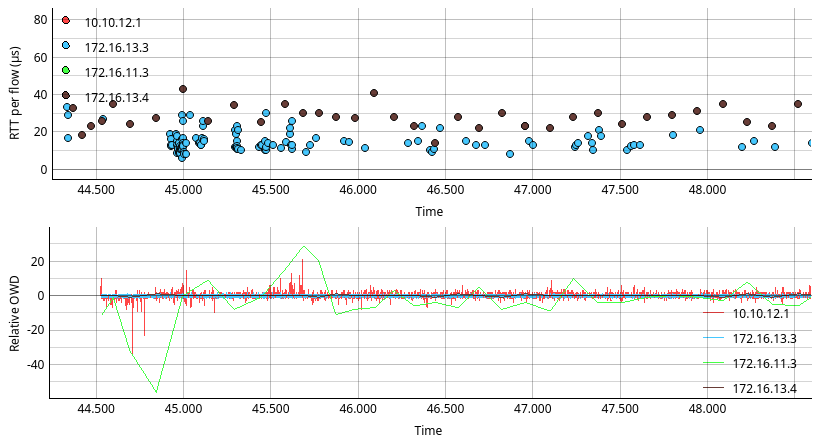
\includegraphics[width=.9\linewidth]{figures/nethint.png}
\caption{\label{fig:orgef50867}Screenshot of NETHINT}
\end{figure}

When running NETHINT, it is possible to make it render a GUI which shows the data as in Figure \ref{fig:orgef50867}. But for our analysis, it is easier to have all this data collected in a file instead. NETHINT supports logging all data into a JSON file by running it with the flag \texttt{-l}, which we then can use for our analysis of the data.

Unfortunately, we later found that this yielded very few packets to be collected by NETHINT. It would therefore likely yield better results to capture a pcap file for the traffic on Router 1s WiFi card, and then analyze this data with NETHINT later. This could be done either by using tcpdump, or by running NETHINT with the \texttt{-w} flag which enable writing to a pcap file. As we did not get the opportunity to run these tests again with this change, we use the pcap files generated by TEACUP on the network interfaces of both Client~1 and Client~2. This should produce similar data except that we cannot guarantee that the real time clocks of the two clients are perfectly synchronized.

It was also found that out of all 192 test runs, 13 of them seem to have failed as no packets were sent between Server~2 and Client~2 apart from SYN and ACK. Upon inspecting the pcap files generated at Client~2, it appears that a TCP RST packet got sent, stopping the TCP transmission. It is unclear why these tests failed, but when using the data in the next sections, we will be excluding these tests. All failed tests had configured delay of 10ms and were the following:

\begin{itemize}
\item 0.5 BDP and VoIP plus one flow each of BBR, Cubic and Reno with bottleneck at WiFi AP
\item 0.5 BDP and three Cubic with bottleneck at WiFi AP
\item 1 BDP and one flow each of BBR, Cubic and Reno with no common bottleneck
\item 1 BDP and VoIP plus three BBR with no common bottleneck
\item 1 BDP and three BBR with no common bottleneck
\item 1 BDP and three Reno with no common bottleneck
\item 1.5 BDP and VoIP plus flow each of BBR, Cubic and Reno with no common bottleneck
\item 1.5 BDP and three Cubic with no common bottleneck
\item 2 BDP and one flow each of BBR, Cubic and Reno with no common bottleneck
\item 2 BDP and VoIP plus three BBR with no common bottleneck
\item 2 BDP and VoIP plus three Cubic with no common bottleneck
\item 2 BDP and three BBR with no common bottleneck
\item 2 BDP and three Reno with no common bottleneck
\end{itemize}
\section{Changes made to NETHINT}
\label{sec:org038d82d}
In order to calculate the correlation between the network streams, we needed to make a few small changes to the NETHINT program. We also found a miscalculation which had to be fixed. These changes were:

\begin{itemize}
\item Enabled logging of the raw OWD, rather than solely the variations in OWD.
\item Corrected the OWD calculation.
\item Modified the program to save information about all packets, not just those with a valid RTT.
\end{itemize}

NETHINT produces JSON files, each with a JSON object representing the data for an individual packet. Within each object, there is information about the destination and source IP addresses and ports, alongside data pertaining to RTT and OWD among other details. Initially, the program was designed to save only the packets for which it could calculate an RTT. However, other metrics, such as OWD, may still be valuable even when RTT data is unavailable. The way that NETHINT calculates the RTT only works for outgoing traffic, which meant that it did not log any packets belonging to incoming traffic. Consequently, we have made certain modifications to NETHINT that expand the range of data it logs. These changes are available at \cslcitation{7}{[7]}. To achieve this, it was only one line which had to be changed:

\begin{verbatim}
- if isset_log() and valid_rtt:
+ if isset_log():
\end{verbatim}

Additionally, there was a mistake in the calculation of the OWD. The OWD is calculated by subtracting the tsval in the timestamp field from the capture time. However, the capture time, which is given by scapy, is given in seconds, while the tsval is in milliseconds, hence, the capture time had to be converted to milliseconds. This was also a rather easy change:

\begin{verbatim}
- owd = self.cap_time - self.tsval
+ owd = int(self.cap_time * 1000) - self.tsval
\end{verbatim}

The value given in tsval is not usually the actual time, but rather a value given by a ``timestamp clock'', nevertheless it should be approximately proportional to real time \cslcitation{8}{[8]}. This means that the calculated OWD is not really the actual time it takes for the packets to travel one way, but that it still is a number that can be used to say something about how the OWD changes. This is fine for our purpose as we are considering how the OWD changes with time, and not the actual values. We still need to have the actual OWD values for our calculations. NETHINT originally only logged how the OWD changed (Current OWD - Previous OWD), however, we need the actual raw OWD values. This meant that we also had to enable logging of the raw OWD values.
\section{Results}
\label{sec:org7201ed4}
In order to compare how the OWD changes between the different bottleneck location configurations, we first calculate the correlation coefficient between the two traffic paths (Server~1 to Client~1 and Server~2 to Client~2). For this we collect the data from the JSON objects by comparing the destination address. This means that we don't differentiate between the different TCP streams between Server~1 and Client~1, but that we look at all data going towards Client~1 as a whole. This gives us two datasets, one for traffic towards Client~1 and one of traffic towards Client~2, allowing us to compare how the OWD changes over time between the two logical topologies in Figure \ref{fig:orga947e73}.

When calculating the correlation coefficient between these two datasets, we get a number representing how much they move together. That is, when one dataset increases, how much does the other increase. In order to calculate this, it is necessary that both datasets are of equal length and have corresponding x values. This is almost guaranteed not to be the case. To solve this, we interpolate the smaller dataset using numpy, by setting:
\begin{lstlisting}[basicstyle=\ttfamily\footnotesize,breaklines=true,showstringspaces=false,postbreak=\mbox{$\hookrightarrow$\space},tabsize=2,language=Python,numbers=none]
y2 = np.interp(x1, x2, y2)
\end{lstlisting}
where \texttt{x2} and \texttt{y2} correspond to the x and y values of the smaller dataset, while \texttt{x1} are the x values of the larger dataset.

After interpolating the dataset, we calculate the correlation coefficient using \texttt{scipy.stats}:
\begin{lstlisting}[basicstyle=\ttfamily\footnotesize,breaklines=true,showstringspaces=false,postbreak=\mbox{$\hookrightarrow$\space},tabsize=2,language=Python,numbers=none]
corr, _ = stats.pearsonr(y1, y2)
\end{lstlisting}

We calculate this correlation coefficient for each test. Then we calculate the CDF for the correlations for each bottleneck configuration. This is done using numpy:
\begin{lstlisting}[basicstyle=\ttfamily\footnotesize,breaklines=true,showstringspaces=false,postbreak=\mbox{$\hookrightarrow$\space},tabsize=2,language=Python,numbers=none]
x = np.sort(y_values)
y = np.arange(1, len(x) + 1) / len(x)
\end{lstlisting}

\begin{figure}[htbp]
\centering
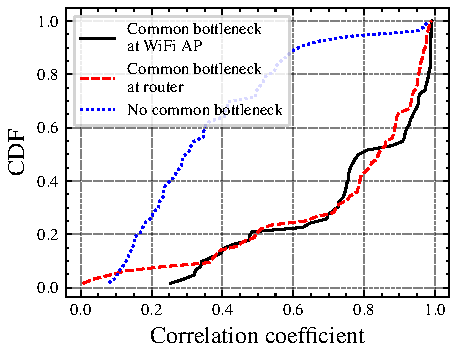
\includegraphics[width=0.7\textwidth]{figures/results/all-over2-no-only-video.pdf}
\caption{\label{fig:org88c0208}CDF graph for all tests}
\end{figure}

Figure \ref{fig:org88c0208} shows the CDF for the correlation coefficient for all the tests. It shows that there is a clear difference in how the OWD changes over time between when the two traffic routes have a common bottleneck and when they do not. It can also be seen that if the correlation coefficient is greater than 0.7, it is very likely that there is a common bottleneck. However, there are still some tests where also the configuration with no common bottleneck have a very high correlation coefficient, showing that this value being high does not guarantee that there is a common bottleneck.

\begin{figure}[htbp]
\centering
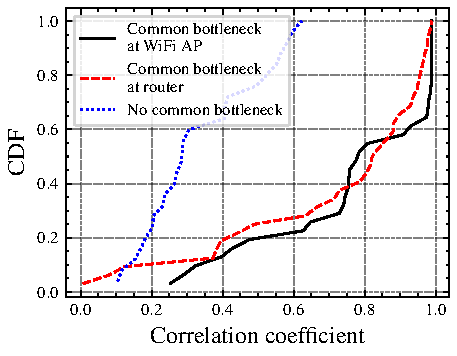
\includegraphics[width=0.7\textwidth]{figures/results/all-over2-no-video.pdf}
\caption{\label{fig:orgee47d20}CDF graph for all tests without VoIP traffic}
\end{figure}

An interesting aspect is that all tests where the correlation coefficient for no common bottleneck in Figure \ref{fig:org88c0208} was above 0.7, also had VoIP traffic between Server~1 and Client~1. When excluding all tests that also had VoIP traffic between these, the highest correlation coefficient for the ``no common bottleneck'' case was 0.62. The entire CDF plot for this is shown in Figure \ref{fig:orgee47d20} where we can see a clear gap between the highest correlation values for when there is no common bottleneck and when there is.
\subsection{Only VoIP traffic}
\label{sec:orge548f9f}
\begin{figure}[htbp]
\centering
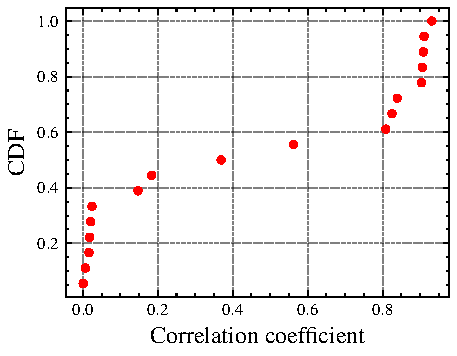
\includegraphics[width=0.7\textwidth]{figures/results/only-video-combined.pdf}
\caption{\label{fig:org557a00e}CDF graph for traffic only containing of VoIP traffic}
\end{figure}

A possible explanation for why having VoIP traffic between Server~1 and Client~1 causes such high correlation could be that having identical traffic patterns directed towards both clients at simultaneously can make it seem more correlated than it should be, despite the presence of other concurrent traffic. We also ran some tests, which are not part of the tests used in Figure \ref{fig:org88c0208}, with just VoIP traffic between Server~1 and Client~1, meaning that the traffic going to the two Clients should be now identical. When only running VoIP traffic like this, we did not generate enough traffic to reach any of the configured throughput bottlenecks, meaning that essentially all tests like this were without any common bottleneck. For this reason, we have combined all the tests into just one CDF plot shown in Figure \ref{fig:org557a00e}, which shows that this traffic tends to seem either very correlated or not very correlated at all, which confirms that the type of traffic being similar can be enough to get very high correlation values.
\subsection{Correlation of CDF}
\label{sec:orgb5ed832}
\begin{figure}
  \centering
  \begin{subfigure}{0.49\textwidth}
    \centering
    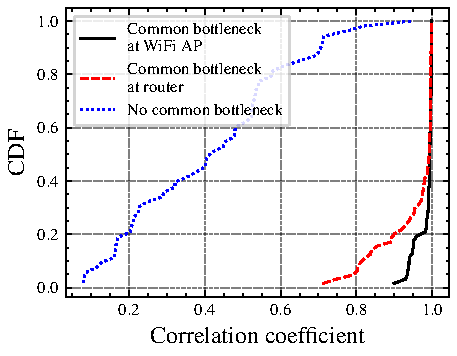
\includegraphics[width=\textwidth]{figures/double-cdf/double-cdf-all-over2-no-only-video.pdf}
    \caption{\label{subfig:double-cdf-all}All data}
  \end{subfigure}%
  \hfill
  \begin{subfigure}{0.49\textwidth}
    \centering
    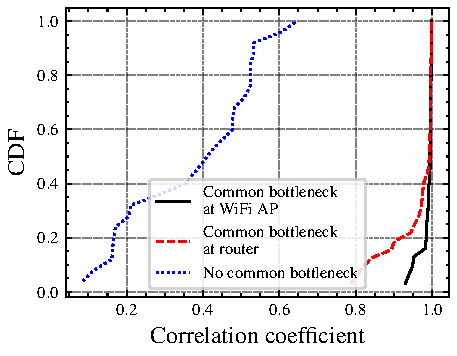
\includegraphics[width=\textwidth]{figures/double-cdf/double-cdf-all-over2-no-video.pdf}
    \caption{\label{subfig:double-cdf-novideo}No tests with VoIP}
  \end{subfigure}%
  %% \caption{\label{fig:double-cdf}CDF data for correlation of CDF}
\caption{\label{org4a725ff}CDF of correlation coefficients of CDF}
\end{figure}

Another way to compare the traffic is to first calculate the CDF for the raw OWDs for traffic directed towards the two Clients. This allows for comparing the distribution of OWD values instead of how the OWD values changes over time. Since the OWD values are not actual real clock time, they will vary significantly in actual values. It is therefore necessary to align the OWD values. We have done this by shifting all OWD values such that the lowest OWD value for each client becomes 0. This means that all other OWD value essentially represent how much longer the OWD is compared to the lowest OWD, and that the calculated correlation represent how similar this distribution is between the two clients. In a practical system, this would be similar to determining the correlation after carrying out long-term measurements covering various traffic patterns.

As can be seen in Figure \ref{org4a725ff} this did not significantly affect the CDF for no common bottleneck, except for decreasing the highest CDF values slightly compared to in Figure \ref{fig:org88c0208}. However, the values for both configurations with a common bottleneck now appear significantly more correlated. With this calculation, the highest correlation coefficient for no common bottleneck is less than 0.95, while this same value only accounts for about 20\% of the tests with a common bottleneck.

When doing the calculation in this way, the difference between including the tests with VoIP traffic, and not including it, was not very significant. This can be seen as the two graphs \ref{subfig:double-cdf-all} and \ref{subfig:double-cdf-novideo} are very similar.
\subsection{Comparison between BDP}
\label{sec:org90d92c5}
\begin{figure}
  \centering
  \begin{subfigure}{0.49\textwidth}
    \centering
    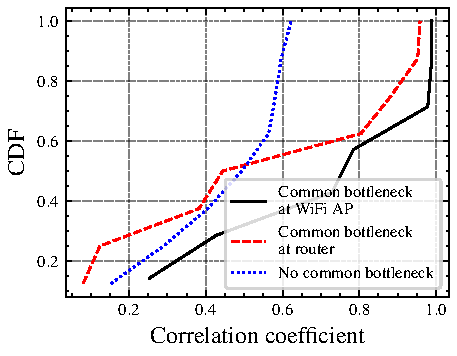
\includegraphics[width=\textwidth]{figures/bdp/bdp-05-no-video.pdf}
    \caption{\label{subfig:bdp-10}0.5 BDP}
  \end{subfigure}%
  \hfill
  \begin{subfigure}{0.49\textwidth}
    \centering
    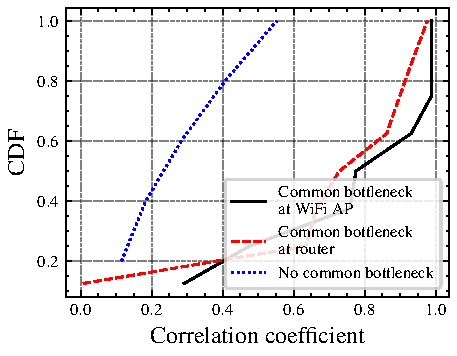
\includegraphics[width=\textwidth]{figures/bdp/bdp-10-no-video.pdf}
    \caption{\label{subfig:bdp-10}1 BDP}
  \end{subfigure}%
  % New line
  \vspace{1ex}
  \begin{subfigure}{0.49\textwidth}
    \centering
    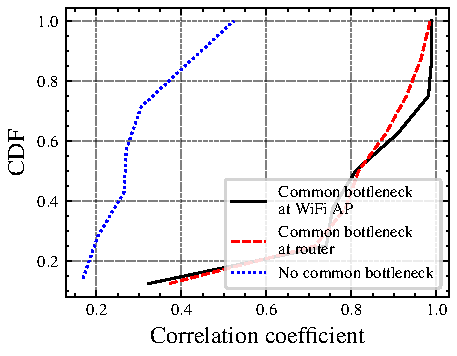
\includegraphics[width=\textwidth]{figures/bdp/bdp-15-no-video.pdf}
    \caption{\label{subfig:bdp-15}1.5 BDP}
  \end{subfigure}%
  \begin{subfigure}{0.49\textwidth}
    \centering
    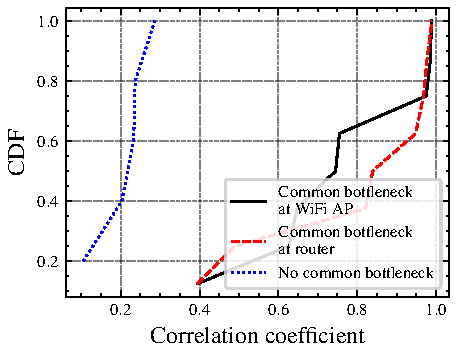
\includegraphics[width=\textwidth]{figures/bdp/bdp-20-no-video.pdf}
    \caption{\label{subfig:bdp-20}2 BDP}
  \end{subfigure}%
  %% \caption{\label{fig:cdf-bdp}CDF plots for each BDP configuration}
\caption{\label{org4d292e6}CDF plots for each BDP configuration}
\end{figure}

Figure \ref{org4d292e6} shows the CDF for each of the BDP configurations separately, rather than the complete data over all configurations that was used for the previous diagrams. This also reflects a more realistic case, as one would typically apply a monitoring tool in one particular network configuration only.

These were calculated as in Section \ref{sec:org7201ed4}, and does not include the tests which also had VoIP traffic from Server~1 to Client~1. It can be seen that the correlations for no common bottleneck tend to decrease as the BDP increases. It is also noticeable how the correlations for when there is a common bottleneck at the router tend to increase as the BDP increases. We don't see the same effect for when the bottleneck is at the WiFi AP, but this is likely due to all the BDP configurations here actually being much smaller as mentioned in Section \ref{sec:org8f1668c}.
\section{Conclusion and future work}
\label{sec:org28da719}
In this assignment, we have demonstrated how NETHINT can be used for determining whether a network bottleneck is situated in the local WiFi or somewhere else by evaluating the OWD of the incoming packets. By calculating the correlation of the OWD of the incoming packets between two clients, we have seen a significant trend in there being a higher correlation when the bottleneck is located in a shared router, rather that when the bottleneck is situated somewhere only affecting the client using the most traffic.

The results were very promising both when correlating how the OWD changes over time, as well as when comparing the distribution of OWD values. But they also showed how the calculated correlation can be high due to similarities in the traffic pattern. This effect of having similar traffic pattern is something that can be further studied in order to better understand its effect on the perceived correlation and how to circumvent it.

In order to properly determine whether NETHINT is suitable for detecting network congestion in a home network, it would also be necessary to run tests with more than two clients as there are likely more devices on a home network.
\section*{References}
\label{sec:orgc57634e}
\begin{cslbibliography}{0}{0}
\cslbibitem{1}{\cslleftmargin{[1]}\cslrightinline{P. J. Barhaugen, “NETwork Home INTerference.” May 08, 2023. Accessed: Nov. 30, 2023. [Online]. Available: \url{https://github.com/petternett/NETHINT}}}

\cslbibitem{2}{\cslleftmargin{[2]}\cslrightinline{S. Zander and G. Armitage, “CAIA Testbed for TEACUP Experiments Version 2,” 2015.}}

\cslbibitem{3}{\cslleftmargin{[3]}\cslrightinline{Oskar, “Ohaukeboe/teacup-nethint.” Dec. 10, 2023. Accessed: Dec. 10, 2023. [Online]. Available: \url{https://github.com/ohaukeboe/teacup-nethint}}}

\cslbibitem{4}{\cslleftmargin{[4]}\cslrightinline{P. Juterud Barhaugen, “Home Network Interference Detection with Passive Measurements,” University of Oslo, 2023.}}

\cslbibitem{5}{\cslleftmargin{[5]}\cslrightinline{M. Mazhar Rathore, A. Ahmad, A. Paul, and S. Rho, “Exploiting encrypted and tunneled multimedia calls in high-speed big data environment,” \textit{Multimed tools appl}, vol. 77, no. 4, pp. 4959–4984, Feb. 2018, doi: \href{https://doi.org/10.1007/s11042-017-4393-7}{10.1007/s11042-017-4393-7}.}}

\cslbibitem{6}{\cslleftmargin{[6]}\cslrightinline{“Manpage of IPERF.” Accessed: Dec. 07, 2023. [Online]. Available: \url{https://iperf2.sourceforge.io/iperf-manpage.html}}}

\cslbibitem{7}{\cslleftmargin{[7]}\cslrightinline{Oskar, “Ohaukeboe/NETHINT.” Dec. 08, 2023. Accessed: Dec. 11, 2023. [Online]. Available: \url{https://github.com/ohaukeboe/NETHINT}}}

\cslbibitem{8}{\cslleftmargin{[8]}\cslrightinline{D. Borman, R. T. Braden, V. Jacobson, and R. Scheffenegger, “TCP Extensions for High Performance,” Internet Engineering Task Force, Request for Comments RFC 7323, Sep. 2014. doi: \href{https://doi.org/10.17487/RFC7323}{10.17487/RFC7323}.}}

\end{cslbibliography}
\end{document}
